\documentclass[12pt]{article}

\usepackage{fancyhdr}
\usepackage{extramarks}
\usepackage{amsmath}
\usepackage{amsthm}
\usepackage{amsfonts}
\usepackage{tikz}
\usepackage[plain]{algorithm}
\usepackage{algpseudocode}

\usetikzlibrary{automata,positioning}

%
% Basic Document Settings
%

\topmargin=-0.45in
\evensidemargin=0in
\oddsidemargin=0in
\textwidth=6.5in
\textheight=9.0in
\headsep=0.25in

\linespread{1.1}

\pagestyle{fancy}

\rhead{\hmwkClass\ : \hmwkTitle}

\lfoot{\lastxmark}
\cfoot{\thepage}

\renewcommand\headrulewidth{0.4pt}
\renewcommand\footrulewidth{0.4pt}

\setlength\parindent{0pt}

%
% Create Problem Sections
%

\newcommand{\enterProblemHeader}[1]{
    \nobreak\extramarks{}{Problem \arabic{#1} continued on next page\ldots}\nobreak{}
    \nobreak\extramarks{Problem \arabic{#1} (continued)}{Problem \arabic{#1} continued on next page\ldots}\nobreak{}
}

\newcommand{\exitProblemHeader}[1]{
    \nobreak\extramarks{Problem \arabic{#1} (continued)}{Problem \arabic{#1} continued on next page\ldots}\nobreak{}
    \stepcounter{#1}
    \nobreak\extramarks{Problem \arabic{#1}}{}\nobreak{}
}

\setcounter{secnumdepth}{0}
\newcounter{partCounter}
\newcounter{homeworkProblemCounter}
\setcounter{homeworkProblemCounter}{1}
\nobreak\extramarks{Problem \arabic{homeworkProblemCounter}}{}\nobreak{}

%
% Homework Problem Environment
%
% This environment takes an optional argument. When given, it will adjust the
% problem counter. This is useful for when the problems given for your
% assignment aren't sequential. See the last 3 problems of this template for an
% example.
%
\newenvironment{homeworkProblem}[1][-1]{
    \ifnum#1>0
        \setcounter{homeworkProblemCounter}{#1}
    \fi
    \section{Exercise \arabic{homeworkProblemCounter}}
    \setcounter{partCounter}{1}
    \enterProblemHeader{homeworkProblemCounter}
}{
    \exitProblemHeader{homeworkProblemCounter}
}

%
% Homework Details
%   - Title
%   - Due date
%   - Class
%   - Section/Time
%   - Instructor
%   - Author
%

\newcommand{\hmwkTitle}{Chapter 2}
\newcommand{\hmwkDueDate}{December 29,2015}
\newcommand{\hmwkClass}{An Introduction to Statistical Learning}
\newcommand{\hmwkClassTime}{}
\newcommand{\hmwkClassInstructor}{G. James et.al.}
\newcommand{\hmwkAuthorName}{Tony Jiang}

%
% Title Page
%

\title{
    \vspace{2in}
    \textmd{\textbf{\hmwkClass:\ \hmwkTitle}}\\
    \normalsize\vspace{0.1in}\small{Due\ on\ \hmwkDueDate\ at 3:10pm}\\
    \vspace{0.1in}\large{\textit{\hmwkClassInstructor\ \hmwkClassTime}}
    \vspace{3in}
}

\author{\textbf{\hmwkAuthorName}}
\date{}

\renewcommand{\part}[1]{\textbf{\large Part \Alph{partCounter}}\stepcounter{partCounter}\\}

%
% Various Helper Commands
%

% Useful for algorithms
\newcommand{\alg}[1]{\textsc{\bfseries \footnotesize #1}}

% For derivatives
\newcommand{\deriv}[1]{\frac{\mathrm{d}}{\mathrm{d}x} (#1)}

% For partial derivatives
\newcommand{\pderiv}[2]{\frac{\partial}{\partial #1} (#2)}

% Integral dx
\newcommand{\dx}{\mathrm{d}x}

% Alias for the Solution section header
\newcommand{\solution}{\textbf{\large Solution}}

% Probability commands: Expectation, Variance, Covariance, Bias
\newcommand{\E}{\mathrm{E}}
\newcommand{\Var}{\mathrm{Var}}
\newcommand{\Cov}{\mathrm{Cov}}
\newcommand{\Bias}{\mathrm{Bias}}

\begin{document}

\maketitle

\pagebreak
1. For each of parts (a) through (d),indicate whether we would generally expect the performance of a flexible statistical learning method to be better or worse than an inflexible method. Justify your answer.\\
(a) The sample size $n$ is extremely large, and the number of predictors $p$ is small.\\
(b) The number of predictors $p$ is extremely large, and the number of observations $n$ is small.\\
(c) The relationship between the predictors and response is highly non-linear.\\
(d) The variance of the error terms, i.e. $\sigma^2$ = Var($\epsilon$), is extremely high.\\
\textbf{Answer:}\\
(a)  better. when the sample size is large and the number of predictor is small, a more flexible provides a better fit
\\
(b) worse. flexible method would suffer from over-fitting. \\
(c) better. more flexible method can better capture the non-linearity relationship.\\
(d) worse. when the data is noisy, flexible method tends to over fit the data which are mostly noise.\\

2. Explain whether each scenario is a classification or regression problem, and indicate whether we are most interested in inference or prediction. Finally, provide $n$ and $p$.\\
(a) We collect a set of data on the top 500 firms in the US. For each firm we record profit, number of employees, industry and the CEO salary. We are interested in understanding which factors affect CEO salary. \\
(b) We are considering launching a new product and wish to know whether it will be a \textit{success} or a \textit{failure}. We collect data on 20 similar products that were previously launched. For each product we have recorded whether it was a success or failure, price charged for the product, marketing budget, competition price, and ten other variables.\\
(c) We are interested in predicting the \% change in the US market, the \% change in the British market, and the \% change in the German market.\\
\textbf{Answer:}\\
(a) regression(inference). n=500,p=3 (number of employees, industry and the CEO salary)\\
(b) classification(prediction). n=20, p=13 (price charged for the product, marketing budget, competition price, and ten other variables)\\
(c) regression(prediction).n=52, p=3(the \% change in the US market, the \% change in the British market, and the \% change in the German market) \\

3. We now revisit the bias-variance decomposition.\\
(a) Provide a sketch of typical(squared) bias, variance , training error, test error, and Bayes (or irreducible) error curves, on a single plot, as we go from less flexible statistical learning methods towards more flexible approaches. The x-axis should represent the amount of flexible in the method, and the \textit{y}-axis should represent the values for each curve. There should be five curves. Make sure to label each one.\\
(b). Explain why each of the five curves has the shape displayed in part (a) \\
\textbf{Answer:}\\
(a)\\
 \begin{center}
 
 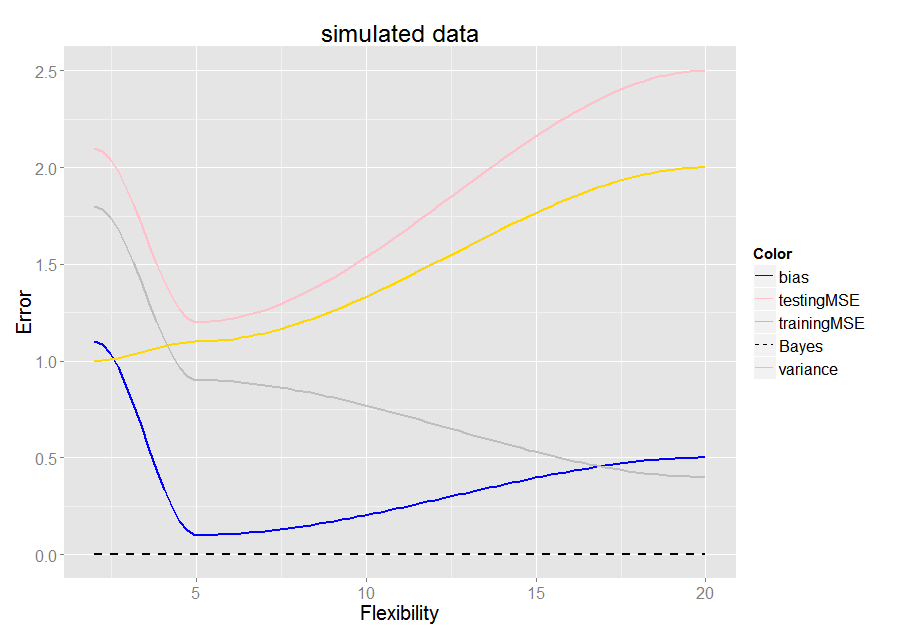
\includegraphics[scale=0.6]{3a.png}
 \end{center}
(b)\\

4. You will now think of some real-life applications for statistical learning:\\
(a) Describe three real-life applications in which \textit{classification} might be useful. Describe the response, as well as predictors. Is the goal of each application inference or prediction? Explain your answer.\\
(b) Describe three real-life applications in which \textit{regression} might be useful. Describe the response, as well as the predictors. Is the goal of each application inference or prediction? Explain your answer.\\
(c) Describe three real-life applications in which \textit{cluster analysis} might be useful. \\
\textbf{Answer:}\\
(a) \begin{itemize}
	\item stock market price direction, prediction, response: up, down,
input: yesterday's price movement % change, two previous day price movement %
change, etc.
\item illness classification, inference, response: ill, healthy, input: resting
heart rate, resting breath rate, mile run time
\item car part replacement, prediction, response: needs to be replace, good,
input: age of part, mileage used for, current amperage
\end{itemize}

(b) \begin{itemize}
\item CEO salary. inference. predictors: age, industry experience, industry,
years of education. response: salary.
\item car part replacement. inference. response: life of car part. predictors: age
of part, mileage used for, current amperage.
\item illness classification, prediction, response: age of death,
input: current age, gender, resting heart rate, resting breath rate, mile run
time.

    \end{itemize}
(c) \begin{itemize}
\item cancer type clustering. diagnose cancer types more accurately.
\item Netflix movie recommendations. recommend movies based on users who have
watched and rated similar movies.
\item marketing survey. clustering of demographics for a product(s) to see which
clusters of consumers buy which products.

    \end{itemize}
5. What are the advantages and disadvantages of a very flexible (versus a less flexible) approach for regression or classification? Under what circumstances might a more flexible approach be preferred to a less flexible approach? When might a less flexible approach be preferred?\\
\textbf{Answer:}\\
The advantages for a very flexible approach for regression or classification
are obtaining a better fit for non-linear models, decreasing bias.

The disadvantages for a very flexible approach for regression or classification
are requires estimating a greater number of parameters, follow the noise too
closely (overfit), increasing variance.
6. Describe the differences between a parametric and a non-parametric statistical approach. What are the advantages of a parametric approach to regression or classification(as opposed to a non-parametric approach)? What are its disadvantages?\\
\textbf{Answer:}\\
A parametric approach reduces the problem of estimating f down to one of
estimating a set of parameters because it assumes a form for f.

A non-parametric approach does not assume a functional form for f and so
requires a very large number of observations to accurately estimate f.

The advantages of a parametric approach to regression or classification are the
simplifying of modeling f to a few parameters and not as many observations are
required compared to a non-parametric approach.

The disadvantages of a parametric approach to regression or classification
are a potential to inaccurately estimate f if the form of f assumed is wrong or
to overfit the observations if more flexible models are used.

7. The table below provides a training data set containing six observations, three predictors, and one qualitative response variable.\\
\begin{table}[ht]
        \centering
        \begin{tabular}{  c | c | c | c | c}
        \hline
          Obs. & $X_1$&$X_2$&$X_3$&$Y$\\
          \hline 
          1 & 0&3&0&Red\\
          2 & 2&0&0&Red\\
          3 & 0&1&3&Red\\
          4 & 0&1&2&Green\\
          5 & -1&0&1&Green\\
          6 & 0&1&1&Red\\
          \hline
            
            
            
        \end{tabular}
    \end{table}\\
Suppose we wish to use this data set to make a prediction for Y when $X_1=X_2=X_3=0$ using \textit{K}-nearest neighbors. \\
(a) Compute the Euclidean distance between each observation and the test point,   $X_1=X_2=X_3=0$\\
(b) What is our prediction with \textit{K}=1? Why?\\
(c) What is our prediction with \textit{K}=3? Why?\\
(d) If the Bayes decision boundary in this problem is highly non-linear, then would we expect the \textit{best} value for \textit{K} to be large or small? Why?\\
\textbf{Answer:}\\
(a) 
\begin{table}[ht]
        \centering
        \begin{tabular}{  c | c | c | c | c|c}
        \hline
          Obs. & $X_1$&$X_2$&$X_3$&$Y$& Distance to (0,0,0)\\
          \hline 
          1 & 0&3&0&Red&3\\
          2 & 2&0&0&Red&2\\
          3 & 0&1&3&Red&$\sqrt{10}$\\
          4 & 0&1&2&Green&$\sqrt{5}$\\
          5 & -1&0&1&Green&$\sqrt{2}$\\
          6 & 1&1&1&Red&$\sqrt{3}$\\
          \hline
            
            
            
        \end{tabular}
    \end{table}\\
(b) Green. The nearest observation is 5. \\
(c) Red. The 3 nearest neighbors are 2,5 and 6 in which Red dominates over Green (2:1)\\
(d) small. needs less neighbors to make the boundary more wiggly. 


\end{document}
